%----------------------------------------------------------------------------
\chapter{A házi feladat megoldása}
%----------------------------------------------------------------------------
%----------------------------------------------------------------------------
\section{Első feladat}
%----------------------------------------------------------------------------
A motort a leírásban részletezett módon modelleztük a PDE toolbox segítségével. Mivel esetünkben, időben változás nincs, így a magnetosztatikai módot választottuk. A motor egyszerűsített modellje egy statorból, rotorból, tekercsekből és légrésből áll. Ezek elrendezését a Matlab parancssorjában adtuk meg, majd mivel az elrendezés a függőleges tengelyre antiszimetrikus, a vízszintesre pedig szimetrikus, így elegendő az egyik negyedet modellezni. A jobb felső negyed kiválasztás után összevontuk a megfelelő elemekhez tartozó subdomaineket, ezután pedig megadtuk az így kialakult peremeken a megfelelő peremfeltételeket. A stator külsejére, illetve a  modell függőleges tengelyre illeszkedő peremére Dirichlet peremfeltételt, mert a peremen a mágneses skalárpotenciál nulla, a modell vízszintes tengelyére illeszkedő peremére pedig Neumann peremfeltételt, mert a mágneses skalárpotenciál normális irányú gradiense nulla. Ezután beállítottuk az adott anyagjellemzőket és az áramsűrűséget a tekercsben. Inicializáltuk a rácshálót, majd a Solve paramétereknél, nemlineáris solvert választottunk adaptív móddal és $ 10^{-11} $ tolarancia határral, az elsőre kiszámolt értékek maximuma $ 10^{-7} $-es nagyságrendbe esett, így a alapértelmezett toleranciahatárra, kevésbé voltak megfigyelhetők a későbbi feladatokban a kisebb változások. 

Látható, hogy a tekercshez közelebb, ahol nagyobbak a mágneses indukció értékei ott a rácshálót is sűrűbben vette fel a program.
 \begin{figure}[!h]
	\centering
	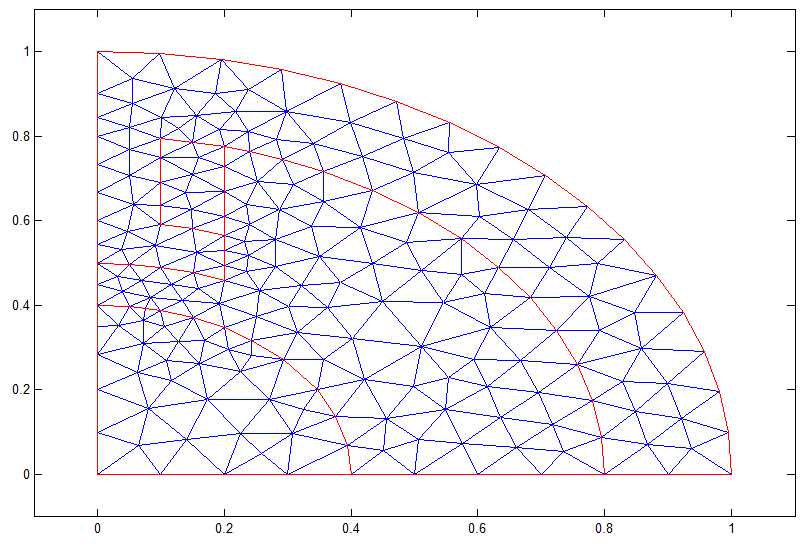
\includegraphics[width=61.5mm, keepaspectratio]{figures/terek/nl_1_init_mesh.png}\hspace{5mm}
	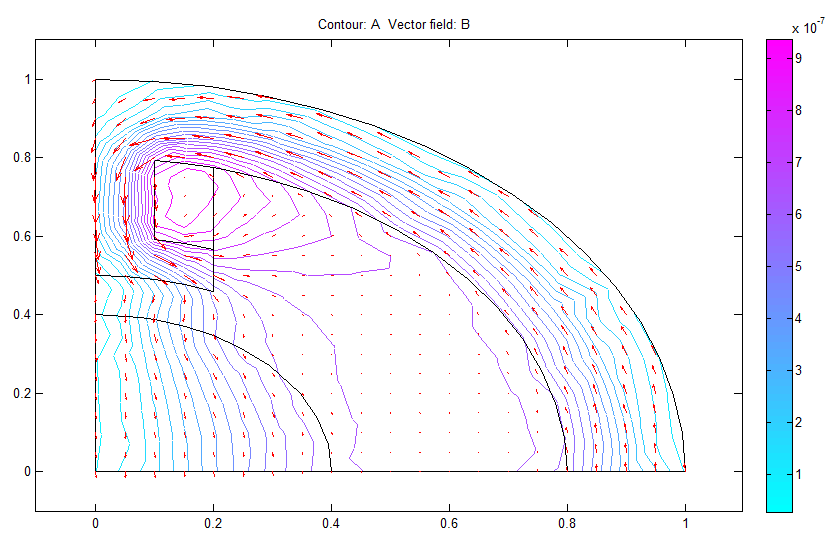
\includegraphics[width=69mm, keepaspectratio]{figures/terek/nl_1_init.png}
	\caption{Az első eredmények}
	\label{fig:calib}
\end{figure}


%----------------------------------------------------------------------------
\section{Második feladat}
%----------------------------------------------------------------------------

A mágneses indukcióvonalak mellett érdemes megvizsgálni, hogy a motoron belül hol mekkora a mágneses indukció abszolútértéke. Ezt mi egy \textit{surface} függvény segítségével ábrázoltuk, mely a \figref{normaleloszlas}~ábrán látható. Miután elvégeztük a modellezést a PDE toolbox segítségével, kiexportáltuk a modellezés során használt háló pontjait, illetve az egyes pontokban a mágneses indukció nagyságát. Az exportált értékeket a \textit{workspace}-ben megjelenítve elkészíthető a 3D-s ábra. Mivel a pontok nem egyenletes távolságra helyezkednek el egymástól, ezért az ábrázoláshoz nem volt lehetséges az ábrázolás egyszerűen csak a \textit{meshgrid} és a \textit{surf} függvények használatával, de a Matlab \textit{griddata} elnevezésű interpoláló függvényével a probléma megoldható. Az abszolút értékek nagyságának leolvasásához egy \textit{colorbar}-t is megjelenítettünk.

\begin{figure}[!h]
	\centering
	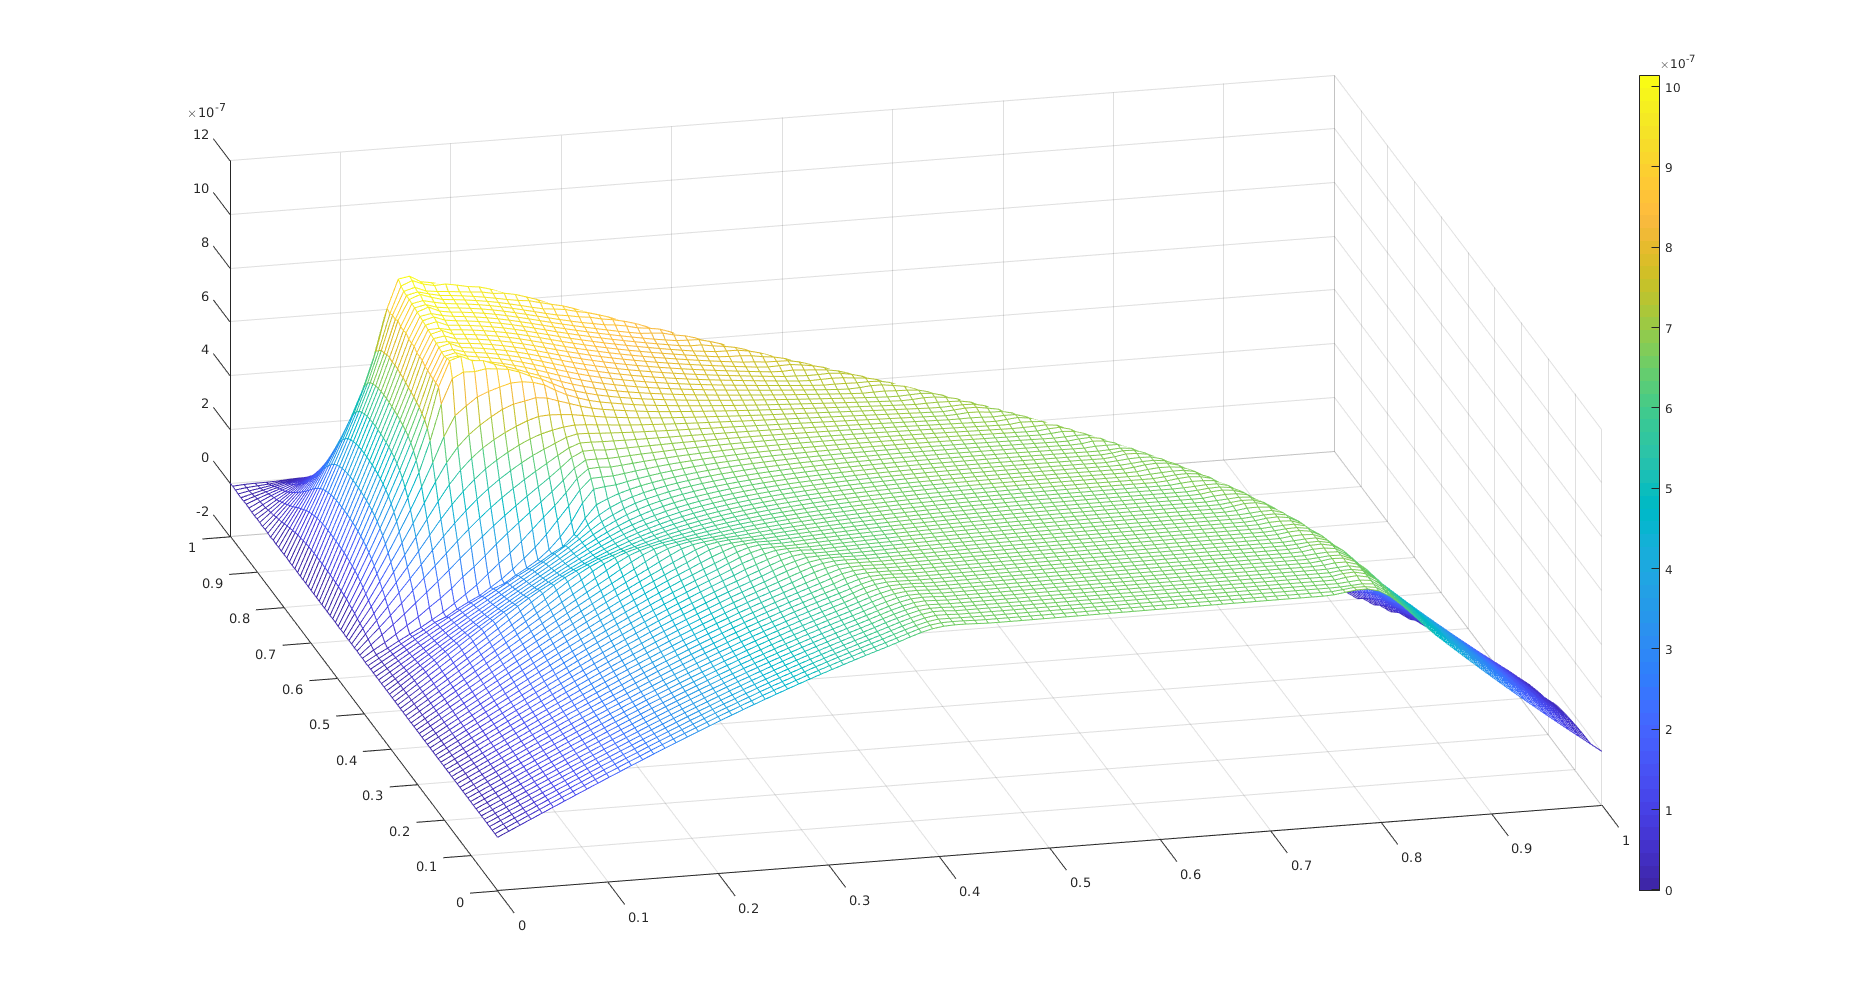
\includegraphics[width=150mm, keepaspectratio]{figures/terek/normal_eloszlas}
	\caption{Mágneses indukció abszolút értékei}
	\label{fig:normaleloszlas}
\end{figure}


Az ábráról leolvasható, hogy a mágneses indukció maximuma  $ 10^{-6} $-on nagyságrendű, és jól látszik, hogy legnagyobb értékek a tekercs közelében tapasztalhatók. Emellett jól megfigyelhető, hogy a stator és a rotor közötti légrésben a tekercstől távolodva a mágneses indukciónak egy „fennsíkja” van, ami kb.  $ 7*10^{-7} $-en értékű. A stator külsején, illetve a függőleges tengely mentén az indukció nagysága 0, ami a peremfeltételekkel összhangban van.
\newpage
%----------------------------------------------------------------------------
\section{Harmadik feladat}
%----------------------------------------------------------------------------
Nemlineáris helyett lineáris vasmagot feltételezve, a modellt így megoldva első ránézésre az indukció abszolút értékeiben nagy változás nem látható, azonban a két felület különbségét képezve az eltérés láthatóvá válik, ezt ábrázoltuk a \figref{kulonbseg}~ábrán.

\begin{figure}[!h]
	\centering
	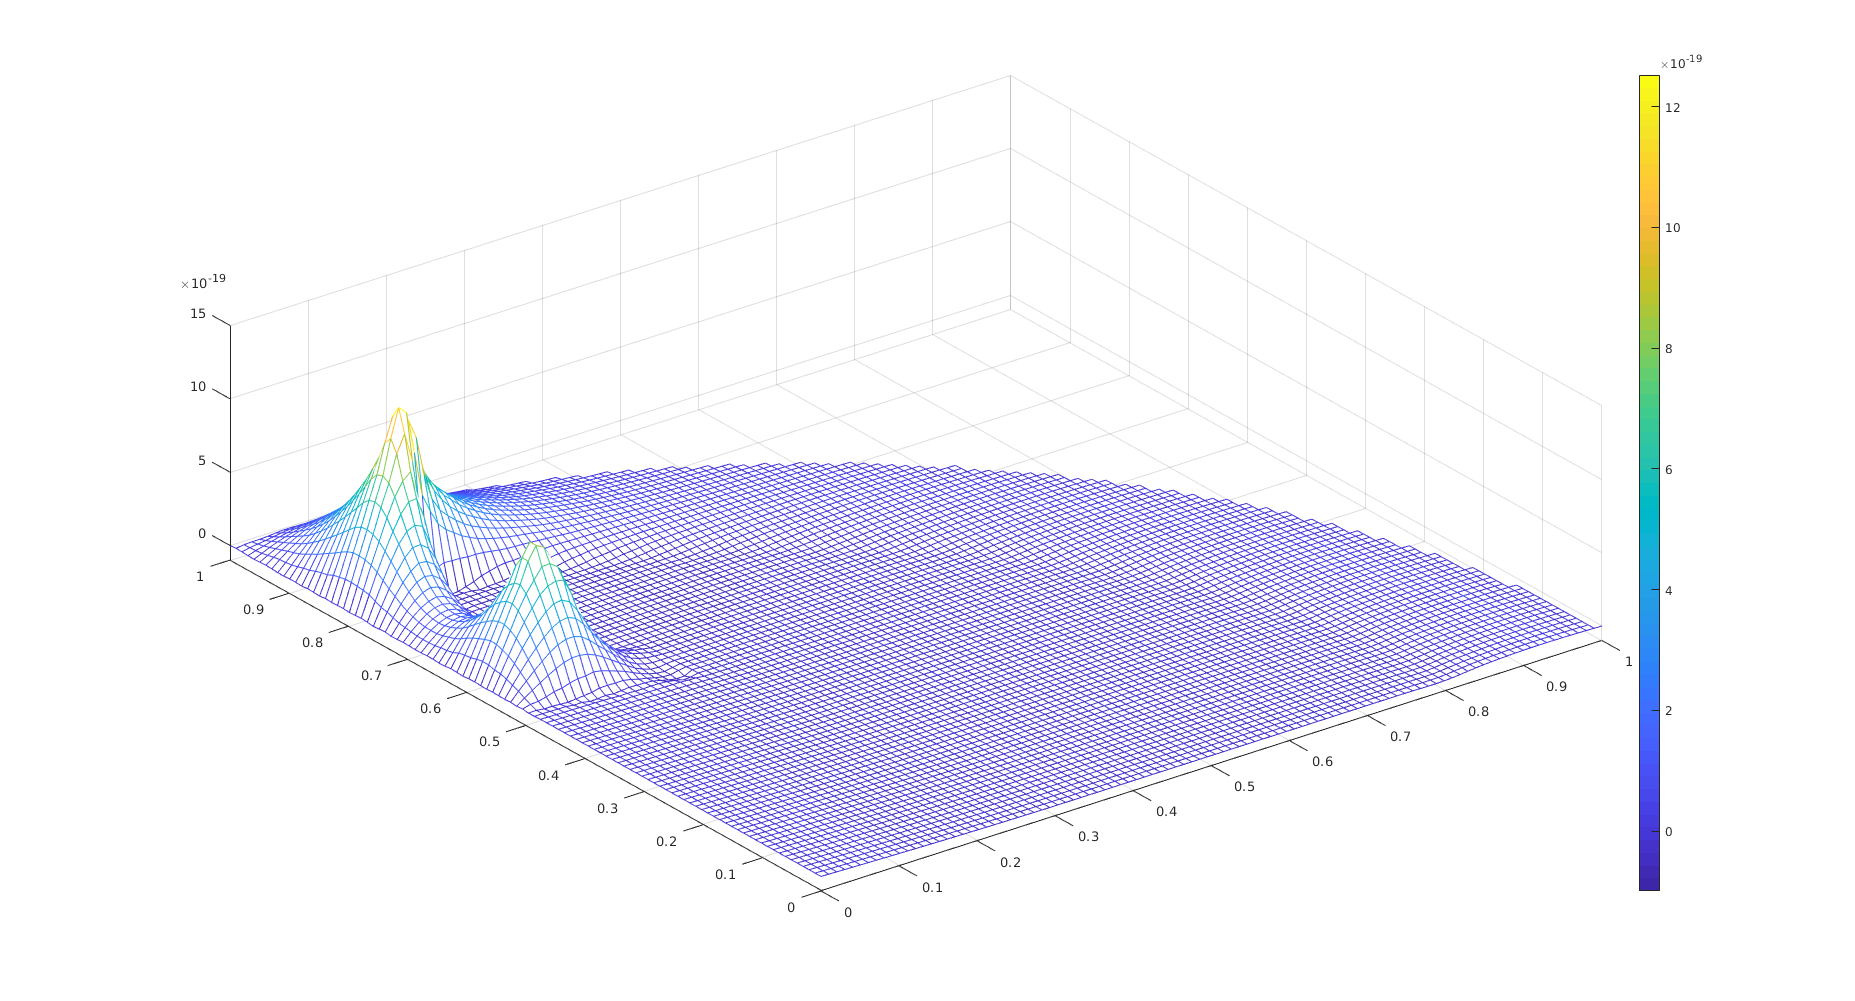
\includegraphics[width=150mm, keepaspectratio]{figures/terek/kulonbseg}
	\caption{A mágneses indukciók nagyságainak különbsége lineáris és nemlineáris vas esetén}
	\label{fig:kulonbseg}
\end{figure}

Megfigyelhető, hogy a legnagyobb eltérés a tekercsnél, azon belül is a tekercs sarkainál tapasztalható. A maximális eltérés a lineáris és a nemlineáris vas között $ 10^{-18} $-on nagyságrendbe esik.




%----------------------------------------------------------------------------
\section{Negyedik feladat}
%----------------------------------------------------------------------------

A PDE ToolBoxban számos lehetőség van a végeselem számítás/(szimuláció?) pontosítására, finomabb végeselemháló készítésére. A háló jóságának egyik jellemzője az őt alkotó háromszögek milyensége. Ez egy 0 és 1 közötti szám, minél nagyobb, annál jobban hasonlít az adott háromszög egy egyenlőoldalú háromszögre. A PDE Toolboxban megtalálható egy \textit{„Jiggle Mesh”} funkció, mely egyenletesebben oszlatja el a csúcspontokat, jobb minőségű háromszögeket alkotva. Ez a funkció a paraméterekben állítható változóval akár többször is lefuttatható, így már a kezdeti háló is javítható a \figref{jiggle} ábrán látható módon.
\begin{figure}[!h]
	\centering
	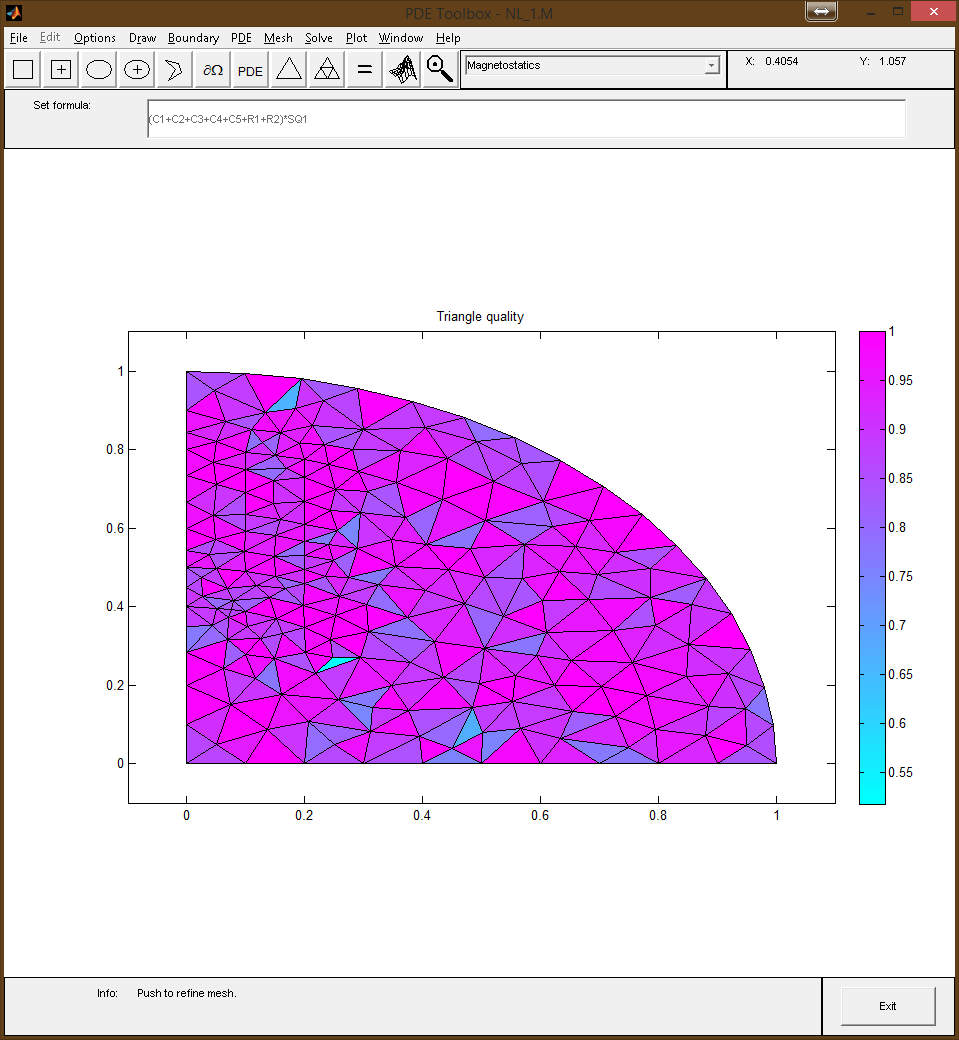
\includegraphics[trim = 25mm 50mm 10mm 70mm,clip, width=69mm, keepaspectratio]{figures/terek/nl_1_3szog0.png}\hspace{5mm}
	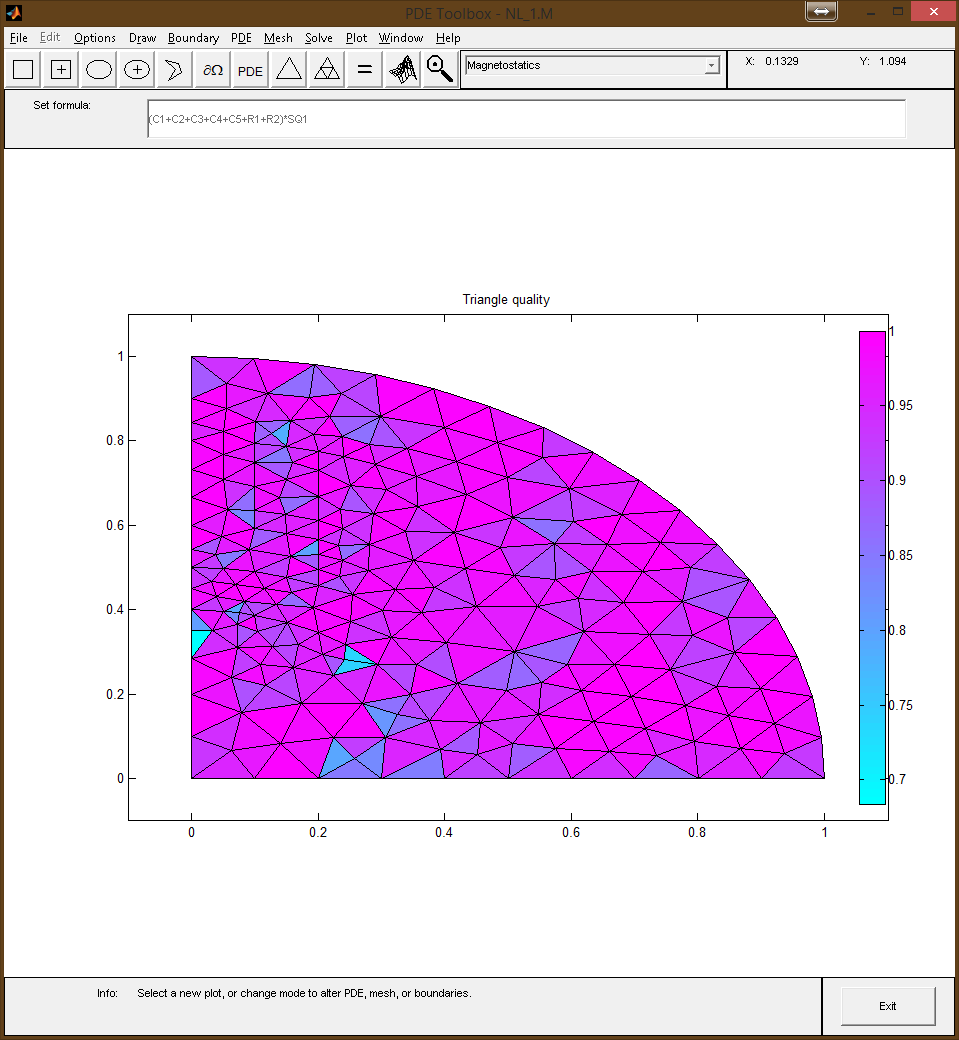
\includegraphics[trim = 25mm 50mm 10mm 70mm,clip, width=67mm, keepaspectratio]{figures/terek/nl_1_3szog1.png}
	\caption{A jiggle nélküli, illetve az azt futtató háló háromszögeinek minőségei}
	\label{fig:jiggle}
\end{figure}

A \textit{„Refine Mesh”} funkcióhoz két paraméter tartozik, az elsővel beállítható, hogy milyen módszerrel finomítsunk a hálón, a másodikkal pedig a növekedési ráta állítható. Az általános esetben a háromszögek oldalainak felezőpontjait összekötve alkot új háromszögeket a toolbox, értelemszerűen így megnégyszerezve az elemek számát, a \textit{longest} módban pedig a háromszög átfogójának felezőpontját a vele szemközti csúccsal köti össze, így megduplázza az elemek számát. Utóbbi módban a növekedési ráta paraméterrel nem csak az eddig meglévő, de már az újonnan létrejött háromszögek egy részén is finomítani lehet egy iteráció alatt.

Ezeken felül lehetőség van az Adaptív végeselemháló finomításhoz, mely a \textit{Solve} paraméterek között kapcsolható be. Itt beállíthatjuk, hogy a szimuláció során mennyi finomítást végezzen a program, azokat milyen módon, illetve mely háromszögekre alkalmazva. A toolbox a legrosszabb minőségű háromszögeket vagy a szomszédos háromszögekhez képest a legnagyobb relatív különbséget elérő(?) háromszögeket finomítja, melyekhez toleranciát is lehet beállítani. Itt több paramétert célszerű kipróbálni, ugyanis túl kis tolerancia esetén az összes háromszögen, túl nagy tolerancia esetén pedig egyiken se fog finomítani az algoritmus. A \figref{adaptive}~ábrán ugyanazon kezdeti hálózat finomítása látható 2 iteráció után, adaptív finomítás nélküli, illetve azt alkalmazó esetben.


\begin{figure}[!h]
	\centering
	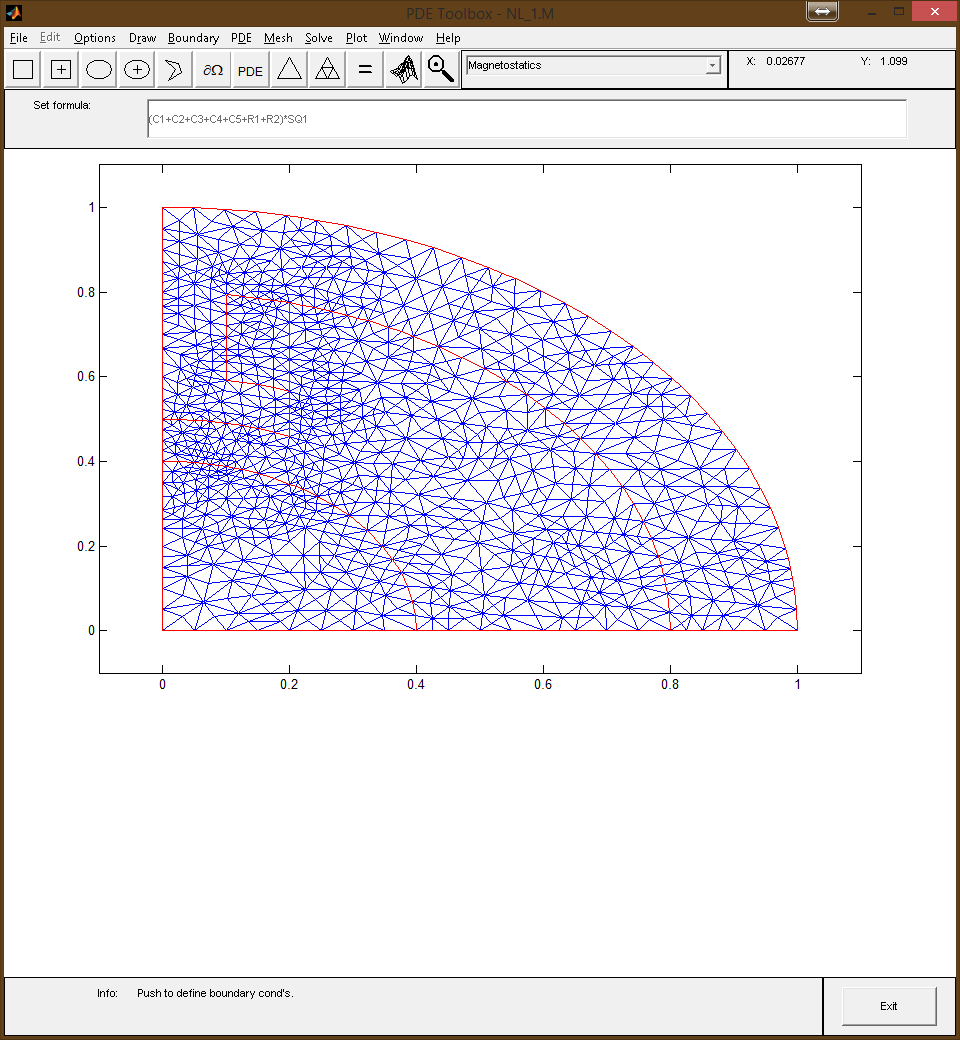
\includegraphics[trim = 15mm 80mm 10mm 40mm,clip, width=69mm, keepaspectratio]{figures/terek/mesh1.png}\hspace{5mm}
	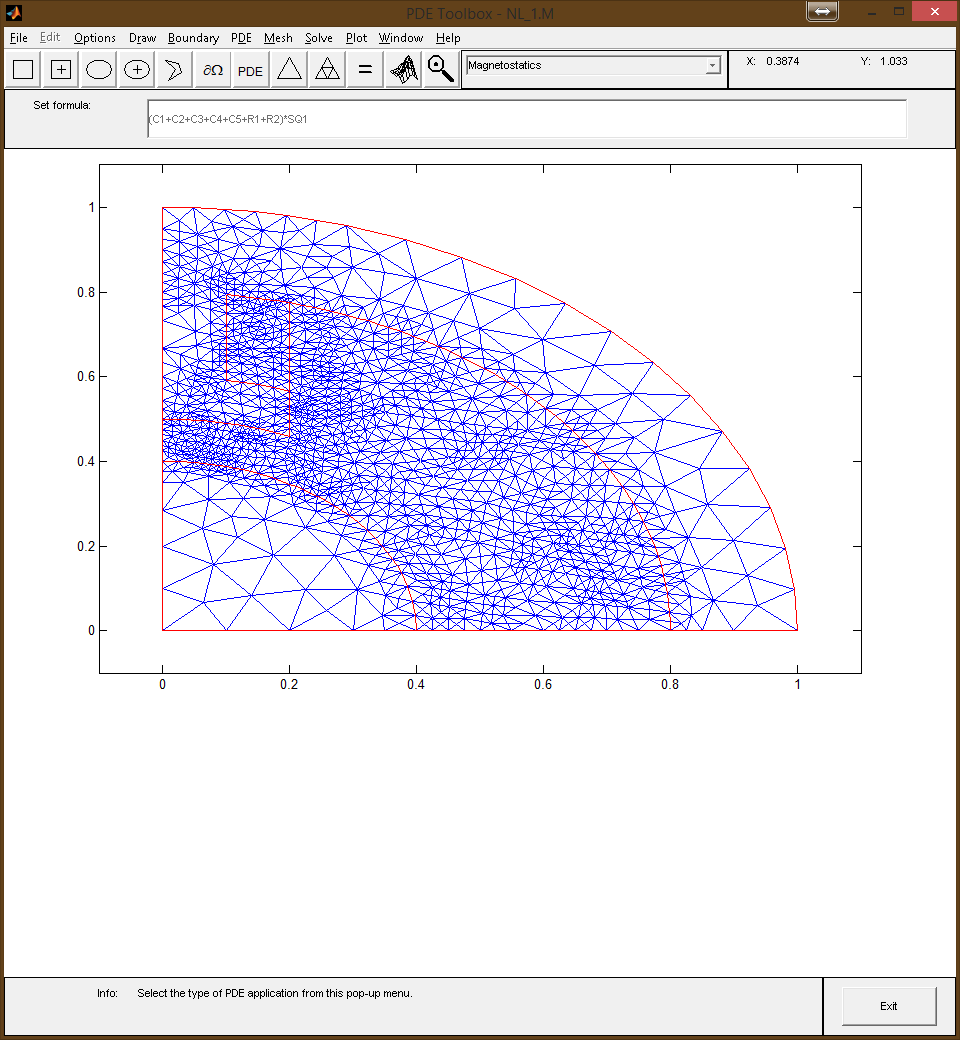
\includegraphics[trim = 15mm 80mm 10mm 40mm,clip, width=69mm, keepaspectratio]{figures/terek/mesh2.png}
	\caption{Adaptív finomítás}
	\label{fig:adaptive}
\end{figure}
\newpage
Ezen ismeretekre alapozva meghatároztunk 4 féle végeselemháló finomítási módot, melyek a következők:


\begin{enumerate}
	\item Nem adaptív, \textit{jiggle} nélküli, \textit{longest} módszerű, 1.3-as növekedési rátával.
	\item Nem adaptív, 20 \textit{jiggle}-t futtató, általános módszerű.
	\item Adaptív, maximum 2000 finomítást, $ 10^{-7} $-es toleranciát használó \textit{longest} módszerű.
	\item Adaptív, maximum 2000 finomítást, $ 10^{-7} $-es toleranciát használó általános módszerű.
\end{enumerate}
Ezeket mind a lineáris, mind a nemlineáris modellre lefuttattuk, az eredményeket kiexportáltuk, és megkerestük a mágneses indukció értékek maximumát. Eredményeink a \tabref{res-lin} és a \tabref{res-nl} táblázatokban találhatóak. Látható, hogy az általános felezőpontos módszer könnyebben megtalálja a felület maximumát, ám az adaptív finomítást használva ez akár lényegesen kevesebb háromszöggel is elérhető.

\begin{table}[!h]
	\centering
	\begin{tabular}{|c||c|c|c|c|}
		\hline
		\textbf{$ *10^{-6} $}		&1. mód&    2. mód&    3. mód&    4. mód\\ \hline\hline
		Inicializáció&   0.96196865034802&   0.96312399284637&   0.98312171335652&   0.98320005165117\\ \hline
		1. Iteráció&   0.97675147818946&   0.98320723184013&   0.98777832396964&   0.99108471276693\\ \hline
		2. Iteráció&   0.98299702428866&   0.99109788082421&   0.99140497343270&   0.99418851293672\\ \hline
		3. Iteráció&   0.98886512022438&   0.99420673120022&   0.99341595180488&   0.99544815538382\\ \hline
		4. Iteráció&   0.99132744744480&   0.99546873795444&   0.99443044519884&   0.99595287564214\\ \hline
		
	\end{tabular}
	\caption{A mágneses indukció maximumértékének változása lineáris modell esetén}
	\label{tab:res-lin}
\end{table}

\begin{table}[!h]
	\centering
\begin{tabular}{|c||c|c|c|c|}
	\hline
	\textbf{$ *10^{-6} $}		&1. mód&    2. mód&    3. mód&    4. mód\\ \hline\hline
	Inicializáció&   0.96196865034802&   0.96312399284635&   0.98312171335651&   0.98320005165113\\ \hline
	1. Iteráció&   0.97675147818948&   0.98320723184012&   0.98777832396964&   0.99108471276696\\ \hline
	2. Iteráció&   0.98299702428871&   0.99109788082414&   0.99140497343272&   0.99418851293635\\ \hline
	3. Iteráció&   0.98886512022444&   0.99420673120021&   0.99341595180488&   0.99544815538414\\ \hline
	4. Iteráció&   0.99132744744506&   0.99546873795697&   0.99443044519850&   0.99595287564182\\ \hline
	
\end{tabular}
\caption{A mágneses indukció maximumértékének változása nemlineáris modell esetén}
\label{tab:res-nl}
\end{table}

\begin{table}[!h]
	\centering
	\begin{tabular}{|c||c|c|c|c|}
		\hline
				&1. mód&    2. mód&    3. mód&    4. mód\\ \hline\hline
		Inicializáció&371&371&1539&1210\\ \hline
		1. Iteráció&902&1484&2932&3888\\ \hline
		2. Iteráció&2059&5936&5628&12943\\ \hline
		3. Iteráció&4546&23744&10972&46215\\ \hline
		4. Iteráció&9813&94976&21345&154082\\ \hline
		
		
	\end{tabular}
	\caption{A végeselem hálót alkotó háromszögek száma}
	\label{tab:res-size}
\end{table}





















